\chapter{Literature Review}
\section{Zika Virus}
Zika virus is a member of the flaviridae family
and the flavivirus genus, it is related to other mosquito borne viruses such as dengue virus, yellow-fever  virus (YFV)  and west nile virus \citep{doi}.The virus originates from the Zika forest of Uganda and the first case was isolated in 1947 from a rhesus monkey in the forest. Then later in 1954 a human was diagnosed with the virus in Nigeria,\citep{2015zika}. Since then the virus has spread to different parts of the world. 
\begin{figure}[h!]
\centering
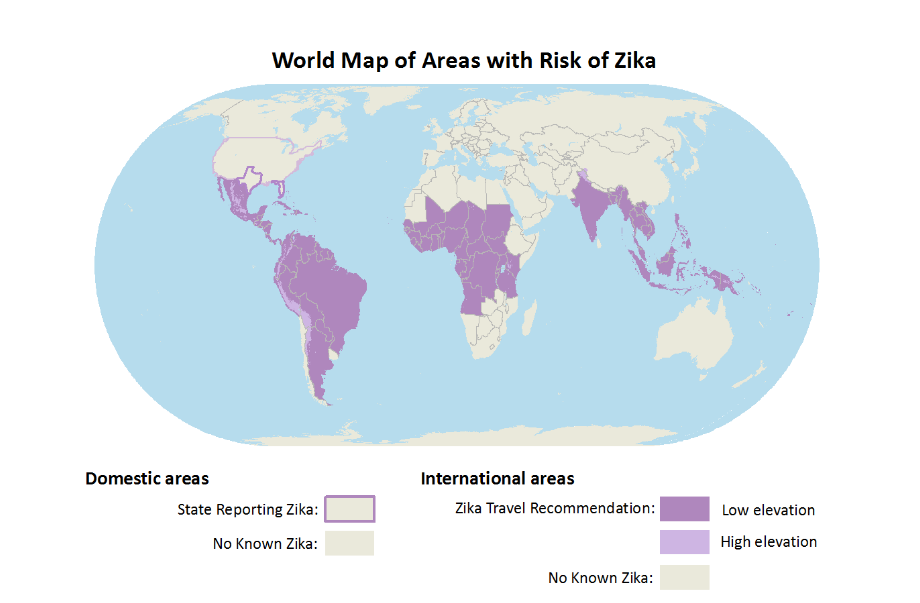
\includegraphics[scale=0.5]{images/map_zika.png} 
\caption{Countries with Zika Virus: Source CDC}\label{fig 1}
\end{figure}


Zika Virus is mainly spread by Aedes mosquitoes. When a pathogen carrying mosquito bites an no infected individual it leaves the pathogen in them. Other ways of by which the virus spreads include, blood transfusion, unprotected sex with an infected person and from mother to child, infected mothers can pass on the virus to their unborn children \citep{musso2014}.

 Some of the symptoms are popular rash,fever,arthritis or arthralgia \cite{musso2015}. In addition, headache, joint pain and red eyes are common symptoms of Zika virus. \cite{simoes2016zika}  adds that pregnant mothers who are infected with Zika during pregnancy usually have child bearing defects. The Zika virus affects their foetus and development of the baby. Babies can face a range of neurologic sequelae such as intellectual disability, hearing loss, vision loss, and seizures. These problems can range from mild to severe and are often life-long \citep{rasmussen2016zika}.

There is no known vaccination to prevent or treat  Zika virus. Prevention measures can be taken to prevent the spread of the virus.This done by preventing mosquito bites. Measures such as sleeping under a mosquito net, using mosquito repellent, spraying mosquitoes inside and outside among others can be taken. Another measure of prevention of Zika virus is practising safe sex and avoiding travel to areas with high prevalence of Zika . Drugs for the symptoms of Zika are administered to patients as a way of treating Zika infected people because of the luck of a vaccination for the virus.


The spread of Zika virus has resulted in Zika epidemics in some part of the world as can be seen in figure \ref{fig 1} above as of April 2017. This causes a worry as the effects of the epidemic are more devastating and if not controlled can affect the whole country, region and World at large. 


 \section{Epidemiology}
 
 Epidemiology is the study of the origin and course of diseases in an community. The goal of epidemiologist is to understand the cause of a disease, then to predict its course, and come up with methods to control the disease.This involves collaborative work by statisticians, mathematicians,physicians and various health specialist \citep{Brauer2017}. The knowledge about infectious diseases has been built up by the method of experience, by observation and analysis of particular conditions associated with occurrence of disease in nature \citep{frost1923importance}.
 
 The first step in epidemiology was collection and analysis of data on causes of death in London parishes in the late 1960s by Graunt. He  gave a method of estimating the comparative risks of dying from various diseases, giving the first approach to a theory of competing risks \citep{Brauer2017}.
 
 Mathematical models for disease transmission have been used to link biological processes of disease transmission and emergence of dynamics of infections at  population level. Researchers try to understand the environmental, biological  and behavioural infectiousness of a disease .
 
  Environmental infectiousness depends on geographical factors of an infected person. Some pathogens cannot survive inside or outside in given conditions. Thus some diseases or infections spread faster in certain weather conditions\citep{grass}. Understanding the timing and causes of seasonality offers important insights on how parasite–host systems interact.How and when parasite control measures can be applied, and how disease risks will respond to anthropogenic climate change and altered patterns of seasonality \citep{altizer}. These factors must be captured in the models.
  
  Biological infectiousness depends on the pathogen's life cycle and the individual's or host's immune system. Some individuals have strong immunity against certain infections, this may  slow down the propagation the infection. On the other hand the life cycle of  pathogens also affect the transmission dynamics of the infection.Some pathogens can only survive in the host while other can survive outside the host, this will play a major role in the spread of the infection.  The interaction of the genetic determinant of disease propagation in the pathogen and host is important in building model for the transmission dynamics of infectious diseases.
  
Behavioural infectiousness depends on the interaction behaviour of an individual. The contact pattern of the person affect how the individual is likely to propagate   the disease. Depending on the nature of disease transmission, a person who has  a lot of contacts is are more likely to spread the disease to more people compared to one who has fewer contacts \citep{johnson2001sexual}. Contact in this context implies any interaction likely to result in transmission of an infection.

The susceptibility of an individual largely depend on the biological, environmental and behavioural factors of an individual. For example one's contact pattern, immunity and the environmental conditions will highly affect the probability of contracting an infection.

Epidemiologist together with mathematicians have for years been involved in infectious disease modelling to understand the dynamics of the spread of the disease and to come with measures of how the spread can be controls. Recently there has been a growing interest in modelling the spread of Zika virus \citep{ku2016}.

Mathematical modelling of infections diseases, started by the works of Daniel Bernoulli in \cite{bernoulli1760essai},in the quest to model the spread of small box and possible eradication. A century later the modelling become well established. The modelling of infectious disease dynamics is important for science and public policy among others. There are three main aims of infectious disease modelling; to is to understand the how the spreading mechanism of the disease, to  predict how the disease will progress among the population and to understand how the disease can be controlled. They provide tools for investigating and quantifying the spread of disease dynamics. Conducting experimental research on the spread of infectious disease raises a lot of ethical issue and therefore can not be conducted on humans. Mathematical simulations and modelling the disease has helped in providing understanding the impact of the infectious disease on the population and give a guide to new control measures \citep{ming2016stochastic}.

Over a  century, Mathematical representation and analysis of infectious diseases has been the centre of  infectious disease epidemiology \citep{b2005}. 
\section{Modelling with Differential Equations.}

Differential equation have been used in the modelling of the dynamics of infectious diseases. They are base on the assumption of uniform mixing, that is everyone in the population has an equal probability of contracting an infectious disease \citep{kaplan2002emergency}.
Compartmental Mathematical models have been used to describe the transmission dynamic of Zika Virus \citep{gao2016}.


 Infectious diseases are transmitted indirectly  or directly by contact between the infected and those who are not infected thus models try to capture these interactions \citep{sat}.Studies have shown that the 
 Susceptible- Infected- Removed(Recovered)(SIR) models and many of its variants have been useful in the modelling of the spread of infectious diseases \citep{li}. Models build on either the SIR or its variants are either deterministic or stochastic. Deterministic models also know as compartmental describe and explains what happens on average of the population. The assume that the population is homogeneous, that is everyone in the population reacts the same to risks of exposure and infection. This assumption in some cases has proved not to realist and hence the introduction of stochastic models. Stochastic models introduce the idea of randomness in the reaction to risk and infection by individual in the population \citep{ming2016stochastic}. The main advantage of the stochastic model is they take into consideration each individual but the major draw back is that it is laborious to model them as they require a lot of simulation and sometimes become mathematically complex.


 
 .To build models that incorporate contact patterns of the individuals, Mathematicians have resolved use to use results from the work of \cite{moreno1945application} where he analysed contact patterns of prisoners. This work give basis for understanding or building models based on the contact patterns of individuals in the population \citep{sat}. \cite{freeman2004development} characterizes the analysis of social networks by four properties. First,it involves the intuition
 that links among social actors 
are important. Second, it is based on the data collection and analysis of data about social relations that link actors.Third,it draws heavily on graphic imagery to reveal and display the patterning of those links and lastly it develops mathematical and computational models to describe and explain those patterns. 
 A number of disease propagation model have being built for various infectious disease among others Malaria, Zika, HIV , Small pox chicken pox \citep{ding2016mathematical}

\section{Modelling with Graph}
Graph theory has over the years grown and has found its application many fields. A graph also known as a network   can be  defined as triple $G = (V,E)$ where $V$ is a finite set of nodes $E \subset V \oplus V = \left\lbrace e_1,e_2,\dots ,e_m \right\rbrace$ is a set  \citep{estrada2012structure}. 

Over the years contemporary science, has had challenges in describing complex networks. This posed limits in the advancement of many disciplines. However, with the advancement  of computerization there is a raise in the possibility of understanding the stability of large networks \cite{barabasi1999emergence} .

For many complex systems vertices are described as elements of the system and edges represent the interaction between them. Similarly, in modelling the spread of  infectious diseases on networks, individuals or populations are represented by nodes of the network, contacts likely to result in the transmission of disease are represented by edges. Modelling of infectious disease on networks give better models for heterogeneous populations \citep{ming2016stochastic}. One of the major challenges is to capture the contact patterns of individuals, the non availability of such data has lead to mathematicians modelling the spread of infectious diseases on various simulated network structures \citep{pastor2001}.

Studying the dynamics of epidemiological models on social networks is currently an active area of research. Many model have been developed on to understand  how the structure of networks affects disease spread \citep{keeling2005networks}.

A number of infectious disease models have been built on various network structures. This is so because networks capture the contact patterns in a community. The networks are either social networks or simulated networks. Many real world and social networks in which infectious disease propagate are either small world or scale free networks and not random or regular as earlier assumed \cite{watts1998collective}.

Random network models of infectious disease do nit take into account spatial position of individuals and connections are made at random \citep{keeling2005networks}. The growth rate and and final epidemic size of a disease on a random network are reduced compared with a random mix model. Growth rate in random network is $\tau (n -2) -g$ and the growth rate with random mixing is $\beta -g = \tau \widehat{n} -g$ , where  $\tau$ is the transmission rate across a contact, $n$ and $\widehat{n} $ , the number of contacts in a network and the unit number of contact per unit time in a random mixing model. The reduction in the growth rate is due to two reasons; each infectious individual has been infected by one of its contacts, reducing the number of susceptible $n-1$ and as an infectious individual starts to infect its susceptible contacts it depletes its local environment, regardless of the population prevalence rate, hence limits the rate of disease spread \citep{keeling2005networks}.

Lattice based epidemic models are used to study the spatial and temporal rates of the disease spread in  a spatially distributed host populations \citep{rhodes1997epidemic}. Models built on latices assume that individuals are located as nodes on a regular lattice and connections are made to a collection of near neighbours or each node. For example people may be spread out such that connections are made to their four nearest neighbours, one on the left,right, up and down this is called a Neumann neighbours  or eight neighbours where four diagonal elements are added to the Neuman neighbours and this is called the Moore neighbourhood \citep{lloyd2006infection}.To avoid the effect of the nodes at the end not being connected the last and first neighbours are made neighbours. The spread of influenza is on of the infectious disease that have been modelled based on lattice models \cite{liccardo2013lattice}. 

Simulated network models have been used to model the spread of disease, whose network data is difficult to collect.


 The underlying structure of a network influences  the effect of that the dynamics of epidemics will have on a population. For example in a small world network, where the network has a high clustering coefficient a shorter average distance. A disease is more likely to spread faster than in a random network or a regular network.


Since the emergence of Zika virus epidemic, there have several studies to model the spread of the virus. Most research on Zika has been modelling the propagation of the infectious using compartmental models as can be seen in the work of \cite{1}, \cite{2} and \cite{3}, where the used the SEIR compartmental model with vector to model the propagation of Zika. Their main assumption is a well mixed population. That is the population is assumed to be homogeneous.
 
In this research we will compare the traditional epidemiological model based on the  assumption of a well mixed or homogeneous population and the Small world networks to model the population Dynamics in the spread of Zika Virus. The tradition compartmental models assumes that everyone in the population has the same probability of catching the infection. While  the model built on a small world network assumes that  one infects his close neighbours with a higher probability compared to any other random person in the network \citep{newman2002random}. This is a much more realistic assumption as it captures the contact patterns of individual in the community or network. Zika virus is mainly transmitted through a vector (Mosquito) contact and transmission is in reference to mosquito bite.



